\chapter{Grundlagen}\vspace{1cm}

In diesem Kapitel sind alle wesentlichen Elemente, die f\"ur die Erstellung der Anwendung verwendet wurden, kurz beschrieben. Zun\"achst wird das Paradigma \textit{Accuracy Awareness} n\"aher erl\"autert und dessen Bezug zu dieser Arbeit aufgezeigt. Im Anschluss wird ein \"Uberblick \"uber die verwendeten Technologien gegeben, welcher zu einem besseren Verst\"andnis der \"ubrigen Kapitel helfen soll. 

\section{Accuracy Awareness Data Processing}
Durch die zunehmende Nutzung von Internet, Telekommunikationsdienstleistungen und IT-Netzwerken ist die Anzahl von Servern und deren Stromverbrauch in den letzten Jahren enorm angestiegen. F\"ur eine energieeffiziente Verarbeitung von gro\ss en Datamengen in Rechenzentren, wurde deshalb mit \textit{Accuracy Awareness} ein neues Paradigma integriert. In der heutigen Zeit verwendet gew\"ohliche Hardware einen hohen Anteil ihres Energieverbrauchs f\"ur die Garantie von Fehlerfreiheit. Mit dem Paradigma \textit{Accuracy Awareness} wird versucht, an genau diesem Punkt Einsparungen zu erzielen. Es wird sich dabei zunutze gemacht, dass wichtige Klassen von Anwendungen fehlertolerant arbeiten bzw. gegen\"uber niedrigen Fehlerraten unempfindlich sind. Daraus resultiert die M\"oglichkeit Energie zu sparen, indem die Genauigkeit und Fehlerfreiheit auf ein akkurates Ma\ss {} reduziert wird. Die Voraussetzung daf\"ur ist die Unterscheidung zwischen fehlerfreien und fehlerbehafteten Daten. Dies ist vorallem wichtig, da beispielsweise Steuerinformationen\footnote{Programmcode, Datei-Header} f\"ur einen korrekten Programmablauf nicht fehlerbehaftet sein d\"urfen. Andere Daten k\"onnen hingegen in gewissen Grenzen Fehler enthalten, ohne die Berechnung zu gef\"ahrden. \\
In Abbildung \ref{SoftwareStack} ist der Aufbau einer Software-Architektur, unter Verwendung des Paradigams, dargestellt. Die Architektur besteht aus den vier Ebenen Job/Task, Middleware, Betriebssystem und Hardware. 

\begin{itemize}
	\item Die Job/Task-Ebene ist beispielsweise durch fehlerbehaftete Datentypen, fehlerbehaftetes lesen und schreiben, als auch fehlerbehaftete Kommunikation beschrieben. Auf dieser Ebene sind fehlertolerante Algorithmen implementiert. Diese haben die Eigenschaft, dass sie in ihren Ausf\"uhrungen durch Datenverluste oder fehlerbehafteten Daten nicht beeinflusst werden.
	\item Die Ebene Middleware stellt Schnittstellen f\"ur eine verteilte Speicherung, Kommunikation und die Nutzung fehlerbehafteter Daten zur Verf\"ugung.\\
	 Das f\"ur diese Bachelorarbeit erstellte Programm arbeitet auf genau dieser Middleware Ebene. Dabei sind speziell die beiden Bereiche fehlerbehaftetes Dateisystem und fehlerbehaftetes Netzwerkprotokoll betroffen.
	\item Die Betriebssysstem-Ebene ist f\"ur die Unterscheidung zwischen fehlerbehafteten Speicherseiten sowie die Netzwerk-Kommunikation verantwortlich.
	\item Auf der Hardware-Ebene wird zwischen fehlerfreien und fehlerbehafteten Daten in den Bereichen CPU/Memory, Speicher und Netzwerk unterschieden. Damit die Hardware diese Unterscheidung treffen kann, m\"ussen an ihr geringf\"ugige Modifiktationen vorgenommen werden. 
\end{itemize} 

Durch \textit{Accuracy Awareness} k\"onnen Rechenzentren dauerhaft von ca. 10\% bis 50\% ihres Stromverbrauchs einsparen und damit zus\"atzlich einen wertvollen Beitrag f\"ur den Umweltschutz leisten \cite{Graubner2012Energy-efficient}.

\begin{figure}[!htb]
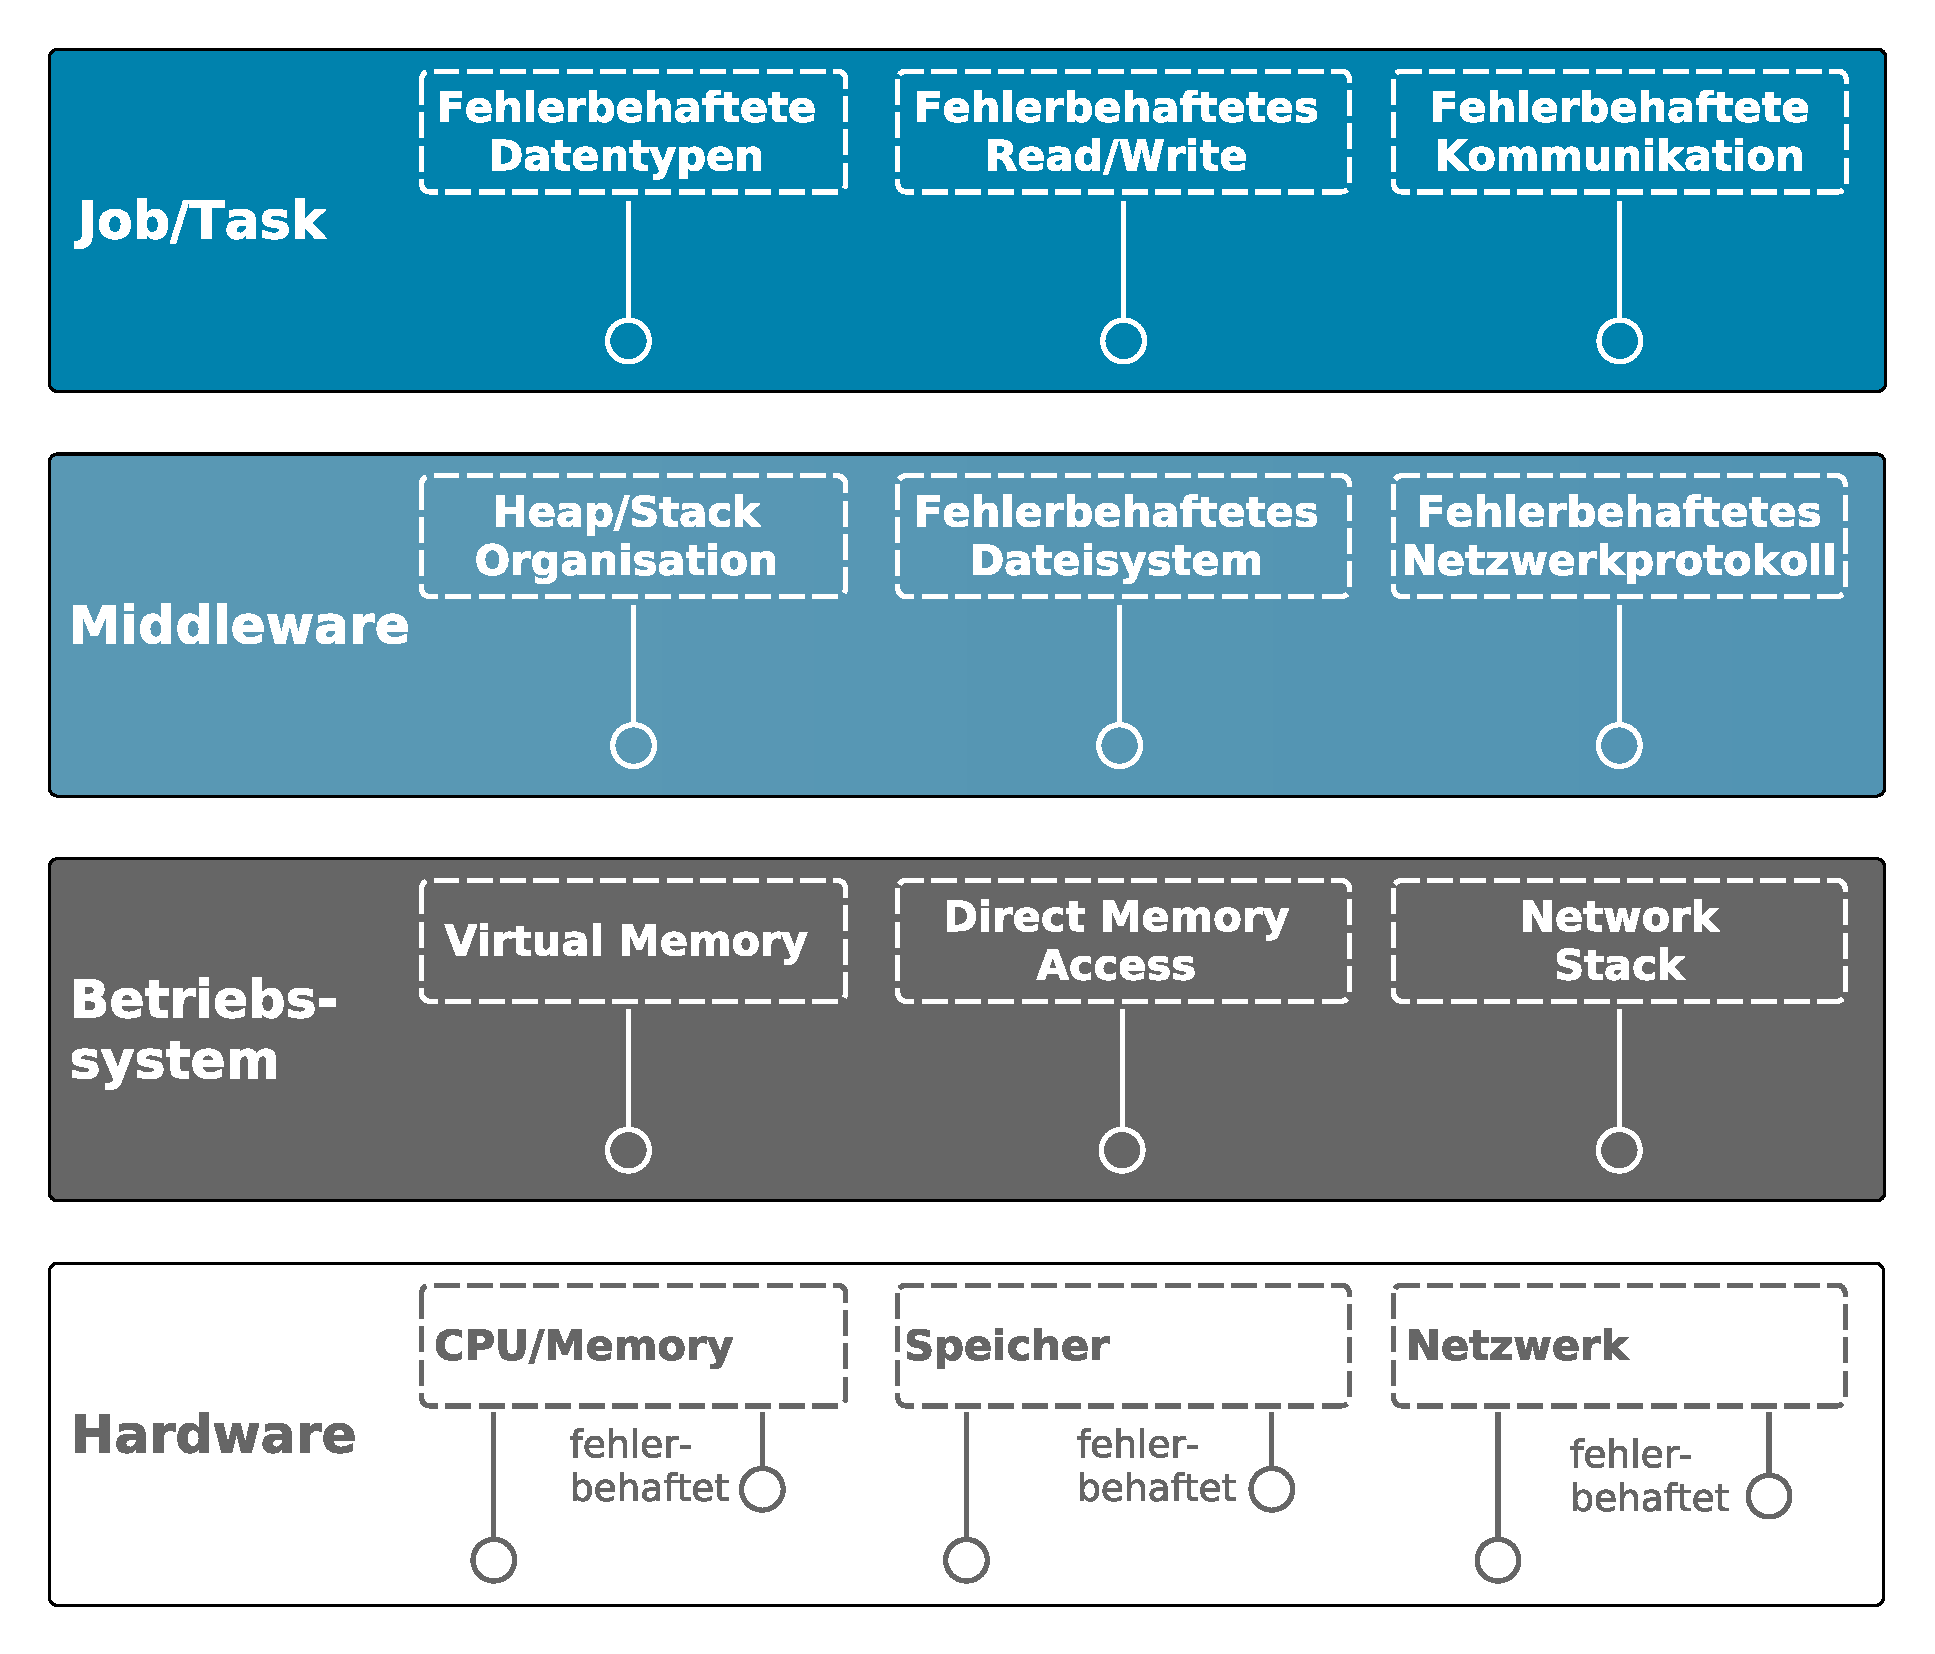
\includegraphics[scale=0.47]{graphics/AccuracyAwareness.eps}
\centering
 \caption[AccuracyAwareness: Software-Architektur]{Software-Architektur \cite{Graubner2012Energy-efficient}}
 \label{SoftwareStack}
\end{figure}

\section{Serialisierung}
Die Objektserialisierung bietet die M\"oglichkeit, Objekte auch ohne Datenbank persistent zu sichern. Dabei wird ein Objektzustand in einen Bytestrom eingepackt. Dieser kann nun problemlos \"uber ein Netzwerk transferiert und auf der anderen Seite wieder ausgepackt werden. Es wird hierbei eine Kopie des aktuellen Objektes zur\"uckgelesen. Um ein Objekt serialisierbar zu machen, muss lediglich das leere Interface \courier{java.io.Serializable} implementiert werden. Die serialisierten Objekte erhalten eine eindeutige Versionsnummer. Tr\"agt ein Objekt eine falsche Versionsnummer kann es nicht deserialisiert werden. Ist keine Nummer angegeben, so benutzt Java einen Hashwert, der sich unter anderem aus den Namen der Klassenattribute errechnet. F\"ur die Deserialisierung wird der Datenstrom eingelesen und ein Java Objekt mit dem gespeicherten Zustand erzeugt \cite{Lange}.

\section{RMI}
RMI\footnote{Remote Method Invocation} bezeichnet einen Mechanismus zur sogenannten verteilten Anwendungsprogrammierung. Vereinfacht ausgedr\"uckt erm\"oglicht es den Zugriff auf Methoden eines entfernten Java-Objekts, welches auf einer anderen Virtuellen Machine und bei Bedarf auf einem anderen vernetzten Rechner l\"auft. Die Details dieses Netzwerkverbundes bleiben dem Aufrufer verborgen, so dass die Arbeit mit verteilten Objekten sich im Prinzip kaum von der mit lokalen Objekten unterscheidet. In Abbildung \ref{RMI} ist diese Funktionsweise grafisch dargestellt.
Auf der Client-Seite nutzt Java sogenannte Stubs zur Kapselung der Daten, welche \"uber das Netzwerk verschickt werden sollen. Ein Stub implementiert das Remote-Interface und dient dem Client als Platzhalter f\"ur das Remote-Objekt. Der Stub kommuniziert \"uber die Netzwerkverbindung mit dem Skeleton auf der Serverseite. Skeletons rufen daraufhin die gew\"unschte Methode auf, \"ubergeben die Parameter und liefern das Resultat an den Client zur\"uck. Sollen komplette Objekt \"ubermitttelt werden, ist die Objekt Serialisierung erforderlich. Objekte, die als Parameter f\"ur RMI-Aufrufe dienen, m\"ussen das Interface \courier{Serializable} aus dem Package \courier{java.io} implementieren.
Die eigentliche Verbindungsaufnahme geschieht \"uber die Serveradresse und einen Bezeichner. Der Bezeichner ist notwendig damit der Namensdienst auf dem Server eine Referenz auf das entfernte Objekt zur\"uckliefern kann. Damit dies funktioniert muss sich das entfernte Objekt zuvor am Server, unter diesem Namen, beim Namensdienst registriert haben. Der RMI-Namensdienst wird \"uber statische Methoden der Klasse \courier{java.rmi.Naming} angesprochen \cite{SBoegel}.

\begin{figure}[!htb]
\centering
\begin{pspicture}(0,0)(35,20)
	\psframe[fillcolor=LLightBlue,fillstyle=solid](0,0)(35,17)
	
	\psframe[](2,17)(9.5,20)
	\psframe[fillcolor=White,fillstyle=solid](2,13.5)(9.5,17)
	\psframe[fillcolor=White,fillstyle=solid](2,7.5)(9.5,13.5)
	
	\psframe[](25.5,17)(33,20)	
	\psframe[fillcolor=White,fillstyle=solid](25.5,13.5)(33,17)
	\psframe[fillcolor=White,fillstyle=solid](25.5,7.5)(33,13.5)
	
	\psframe[fillcolor=White,fillstyle=solid](2,4)(33,7.5)
	
	\rput(28,2){\textbf{{\normalsize RMI}}}
	\rput(5.75,18.5){\textbf{{\normalsize Client}}}
	\rput(5.75,15.25){\textbf{{\normalsize Stub}}}
	\rput(5.75,10.5){\textbf{{\normalsize \parbox[c]{2cm}{Remote\\Reference\\Layer}}}}
	\rput(29.25,18.5){\textbf{{\normalsize Server}}}
	\rput(29.25,15.25){\textbf{{\normalsize Skeleton}}}
	\rput(29.25,10.5){\textbf{{\normalsize \parbox[c]{2cm}{Remote\\Reference\\Layer}}}}
	\rput(17.5,5.75){\textbf{{\normalsize Netzwerkverbindung}}}
	\rput(17.5,18.5){\textbf{Virtuelle Verbindung}}
	\psline{<-}(10,18.5)(12,18.5)
	\psline{->}(23,18.5)(25,18.5)
\end{pspicture}

 \caption[RMI Kommunikations-Architektur]{RMI Kommunikations-Architektur  \cite{SBoegel}}
 
 \label{RMI}
\end{figure}

\section{JMX}
Mittels JMX\footnote{Java Management Extensions} ist es gelungen, Java Anwendungen und Dienste über einen standardisierten Weg zu verwalten und zu \"uberwachen. Die damit entwickelte Spezifikation beschreibt eine Architektur, eine API, Design Patterns, verschiedene Verwaltungsdienste f\"ur Anwendungen sowie Monitoring Dienste f\"ur Java. Durch die Unterst\"utzung von Adaptern und Konnektoren erm\"oglicht JMX die Kommunikation zwischen verschiedenen JVM\footnote{Java Virtual Machine}. Eine Anwendung kann somit beispielsweise \"uber einen einfach implementierten HTTP-Adapter, mittels Webbrowser gesteuert werden. In Abbildung \ref{JMX} sind die verschiedenen Ebenen der JMX-Architektur dargestellt \cite{KKoehler}.\\
Die zu \"uberwachenden Resourcen befinden sich auf der Ebene Instrumentation Level. Sie werden als MBeans\footnote{Managed Bean} repräsentiert. MBeans gibt es in verschiedenen Variationen, wie beispielsweise Standard oder Dynamic MBeans. Damit der Client Zugriff auf die Resourcen bekommt, sind sogennante Agents notwendig. Diese befinden sich auf dem Agent Level\footnote{auch MBeanServer} und sprechen die Resourcen direkt an. Diese Ebene wird deshalb auch als Mittelsmann zwischen Anwendung und den MBeans bezeichnet. Das Distributed Services Level dient als Schnittstelle, um den Zugriff der Management Applikationen auf die Agents, innerhalb des Servers zu erm\"oglichen. Die verbindung wird \"uber sogenannte Connectors oder Adaptors aufgebaut. Der Connector liefert den vollen Zugang zu der MBeanServer API und kann via RMI, JMS die Verbindung herstellen. Ein Adaptor adaptiert die API auf ein anderes Protokoll wie SNMP oder auf webbasierte Oberfl\"achen wie HTML/HTTP, WML/HTTP \cite{JMXOracale}.

\begin{figure}[!htb]
\centering
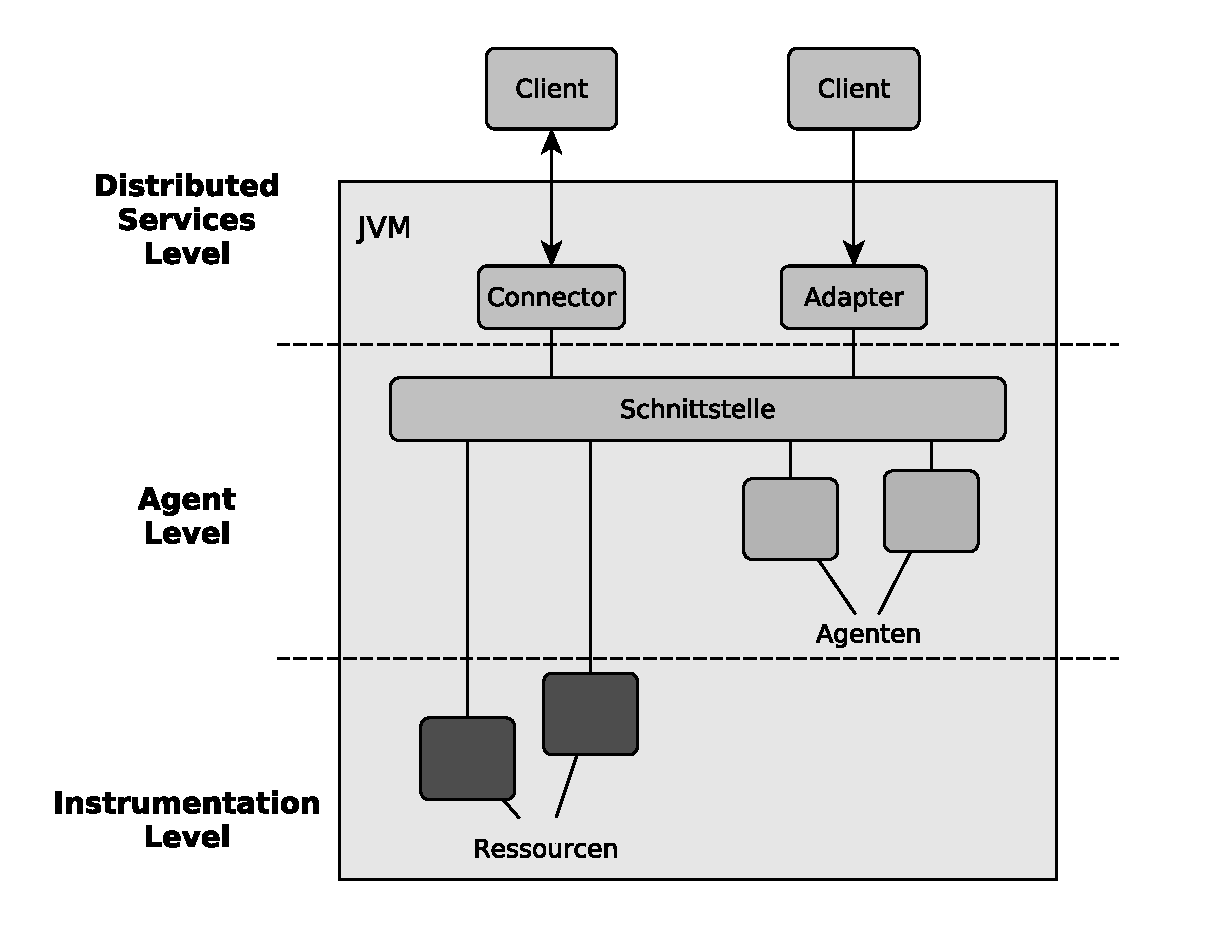
\includegraphics[scale=0.8]{graphics/JMX.eps}
 \caption[JMX-Architektur]{JMX-Architektur \cite{wikiJMX}}
 \label{JMX}
\end{figure}

\section{Jmxtools}
Die Java library Jmxtools stellt eine gro\ss e Auswahl an n\"utzlicher Zusatzfunktionalit\"at f\"ur die JMX Implementierung bereit. In dieser Arbeit wurde die Library f\"ur die Implementierung eines HTML-Clients verwendet. JMXtools bietet zu diesem Zweck einen \courier{HtmlAdaptorServer} an. Dieser erm\"oglicht es einen Zugang auf die Agent-View \"uber einen Webbrowser zu erstellen. Anschlie\ss end k\"onnen die verwalteten Ressourcen \"uber den Webbrowser verwendet werden.  

\section{Javassist}

Javassist\footnote{Java programming assistant: http://www.csg.ci.i.u-tokyo.ac.jp/$\sim$chiba/javassist/}  ist eine Java library mit deren Hilfe sich der Bytecode einer Java Anwendung leicht manipulieren oder neuer Bytecode erstellen l\"asst. Diese Eigenschaft war f\"ur die dynamische Modifikation der Fehlerwerte eine wichtige Voraussetzung.\\ Eine Java Klasse ist, sobald sie in die JVM geladen wurde, nicht mehr ohne weiteres ver\"anderbar. F\"ur diese Bachelorarbeit war es jedoch notwendig die Parameter einer Annotation zur Laufzeit modifizierbar zu halten. Da Annotationen im urspr\"unglichen Sinne, nur f\"ur den Compiler vorgesehen und deshalb auch nur zur Compilezeit ver\"anderbar sind, musste auf Bytecode-Ebene gearbeitet werden. Javassist stellt hierf\"ur die folgenden Operationen bereit.\\
Die wichtigste Klasse ist der \courier{classPool}, indem die zu manipulierenden Klassen eingef\"ugt werden m\"ussen. Anders als der JVM classloader, werden geladene Klassen durch die Javaassist API als Daten verwendbar gehalten. Klassen die in den \courier{classPool} aufgenommen werden, sind Instanzen von \courier{javassist.CtClass}. Eine \courier{CtClass} bietet zus\"atzlich zu den normalen Methoden der Class Datei die M\"oglichkeit neue Methoden, Felder und Konstruktoren der Klasse hinzuzuf\"ugen, sowie Klassenname, Superklasse und Interfaces abzu\"andern. Felder, Methoden und Konstruktoren werden durch \courier{javassist.CtField}, \courier{javassist.CtMethod}, und \courier{javassist.CtConstructor} dargestellt, welche Methoden f\"ur ihre jeweiligen Modifikationen mit sich f\"uhren \cite{JavaAssi}. Der allgemeine Modifikationsablauf ist in Abbildung \ref{Javassist} dargestellt. Hierbei wird die Ausgangsklasse \"uber die Bytecode-Manipulation um neue Aspekte, in Abbildung \ref{Javassist} die um \courier{if}-Anweisung und die \courier{@override} Annotation, erweitert. Die neu geladene Klasse enth\"alt im Anschluss beide Elemente.\\
Javassist bietet damit ausreichend Funktionionalit\"at um die gew\"unschte dynamische Regulierung umsetzen zu k\"onnen, ohne wesentliche Auswirkungen auf die Laufzeit der Anwendung zu haben. In Kapitel \ref{chp:eval} Evaluation, wurde diese Eigenschaft anhand einer Messung belegt.

\begin{figure}[!htb]
\centering
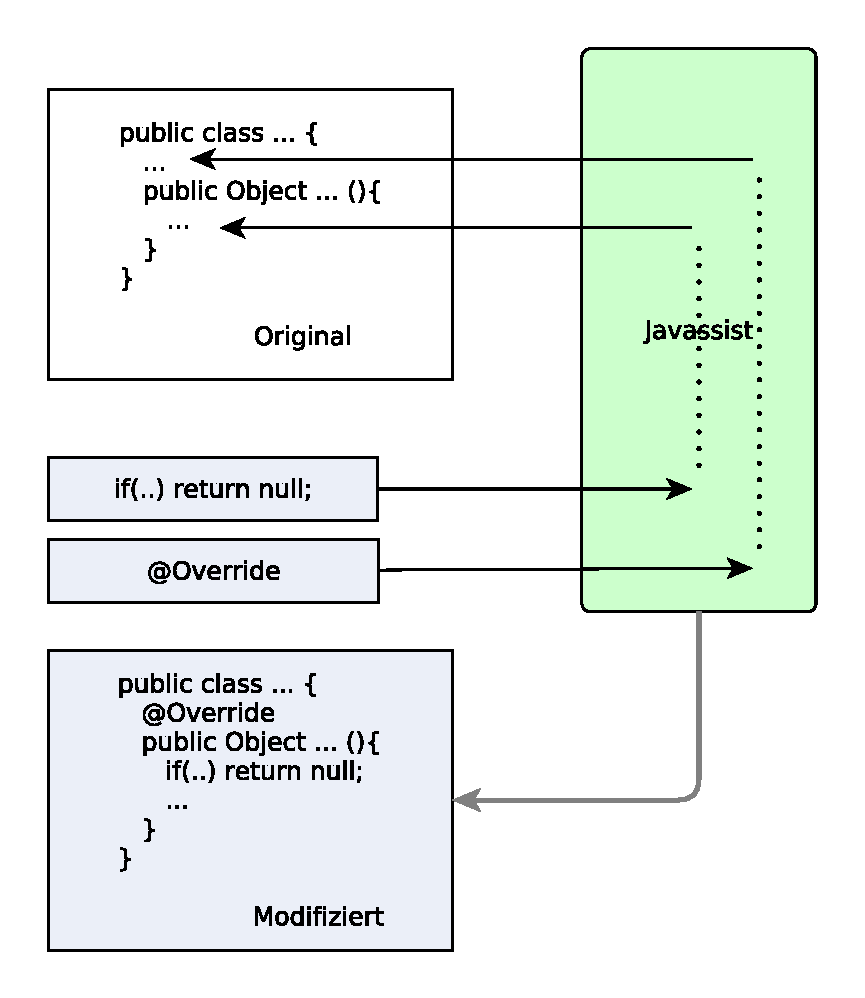
\includegraphics[scale=0.8]{graphics/javassist.eps}
 \caption[Javassist Code-Manipulation]{Code-Manipulation mit Javassist \cite{Huang:2011:SBA}}
 \label{Javassist}
\end{figure}

\section{HotSwapper}
Wie bereits beschrieben ist es durch javassist m\"oglich Klassen w\"ahrend der Laufzeit zu modifizieren und mit den neu erstellten Instanzen zu arbeiten. Sind allerdings bereits Instanzen der jeweiligen Klasse geladen, erh\"alt man die Fehlermeldung: \textit{duplicate class definition}. Um die durch javassist modifizierten Klassen respektive deren modifierzierten Bytecode f\"ur alle involvierten Objekte verwendbar zu machen, wurde \courier{javassist.util.HotSwapper}\footnote{http://www.csg.ci.i.u-tokyo.ac.jp/$\sim$chiba/javassist/html/javassist/util/HotSwapper.html} in die Implementierung eingebunden. Der \courier{Hotswapper} ben\"otigt zus\"atzlich die Einbindung der tools.jar library in den BuildPath und diverse VM-Argumente, die im Abschnitt Konfiguration im Kapitel Design erl\"autert werden. Die Funktionsweise der Klasse \courier{HotSwapper} ist in Abbildung
\ref{Swapper} grafisch dargestellt. Der neue Bytecode wird \"uber den Debugger in die Class Datei des jeweiligen Objektes eingef\"ugt und diese anschlie\ss end neu geladen. F\"ur den Ladevorgang stellt die Klasse \courier{HotSwapper} die Funktion \courier{reload} bereit. Nach dem Update des Bytecodes und dem Ladevorgang, k\"onnen alle betroffenen Klassen den neuen Code, beim Methodenaufruf ausf\"uhren.

\begin{figure}[!htb]
\centering
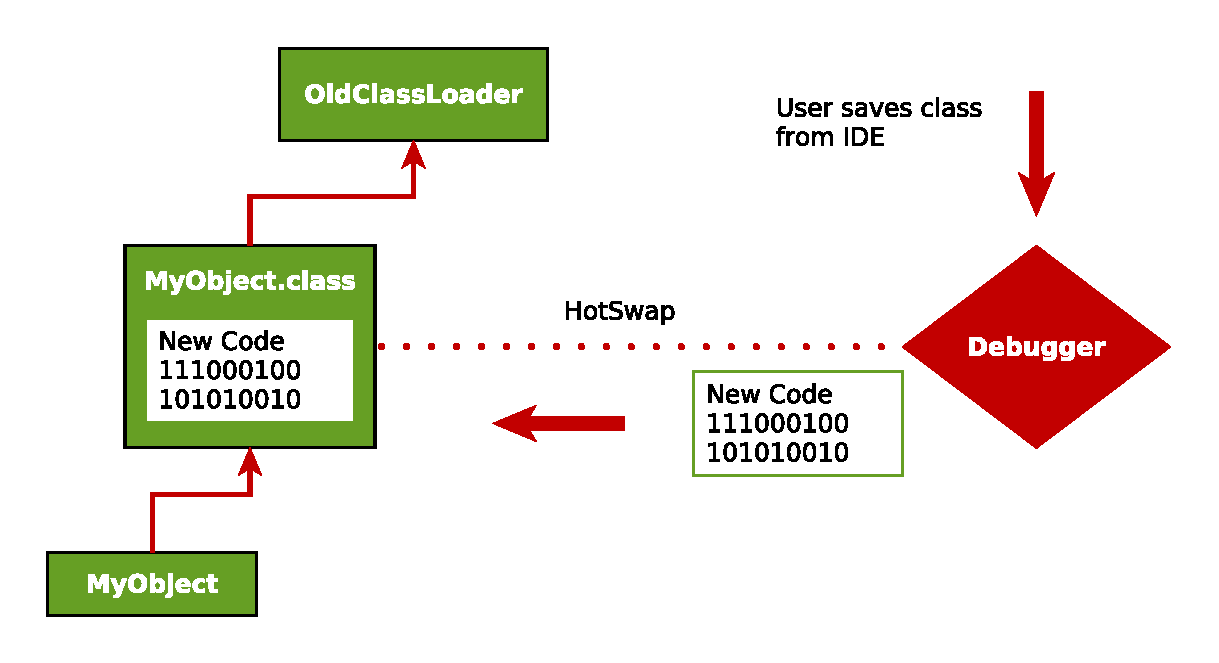
\includegraphics[scale=0.8]{graphics/HotSwapper.eps}
 \caption[Funktionsweise HotSwapper]{Funktionsweise HotSwapper \cite{HotSwapper}}
 \label{Swapper}
\end{figure}